\documentclass[a4paper,12pt]{article}
\usepackage[indonesian]{babel}
\usepackage{graphicx}
\usepackage{longtable}
\usepackage{tabularx}
\usepackage{geometry}
\geometry{a4paper, margin=2.5cm}
\usepackage{hyperref}
\usepackage{multirow}
\graphicspath{{alya_images/}}

\begin{document}

\tableofcontents
\newpage
\listoffigures
\newpage
\listoftables
\newpage

\section{PENDAHULUAN}

\subsection{Latar Belakang}

Diabetes melitus merupakan ancaman kesehatan global paling krusial. Eskalasi jumlah penderita yang terus meningkat setiap tahunnya menempatkan penyakit ini sebagai salah satu penyebab mortalitas tertinggi yang kini mengintai seluruh lapisan masyarakat tanpa batasan usia. Berdasarkan data International Diabetes Federation (2025), sekitar 589 juta penduduk usia dewasa (20–79 tahun) hidup dengan diabetes pada tahun 2024. Pada tahun yang sama, diabetes menyebabkan lebih dari 3,4 juta kematian global dan menghabiskan sedikitnya USD 1 triliun untuk pembiayaan kesehatan (International Diabetes Federation, 2025). Di Indonesia, diabetes semakin mengkhawatirkan dengan sekitar 20,4 juta penyandang diabetes. Lebih memprihatinkan lagi, 73,2\% atau sekitar 15 juta orang dewasa di Indonesia belum terdiagnosis, menempatkan Indonesia di antara negara dengan angka kasus diabetes tidak terdeteksi tertinggi di dunia (International Diabetes Federation, 2025). Kondisi yang lebih parah lagi adalah risiko komplikasi kronis berupa penyakit kardiovaskular, strok, gagal ginjal, retinopati, neuropati, amputasi, hingga kematian dini yang menurunkan kualitas hidup masyarakat serta meningkatkan beban pembiayaan kesehatan nasional (Kumar et al., 2020).

Diabetes melitus telah menjadi masalah kesehatan yang signifikan dan menjadi tantangan utama pembangunan kesehatan global. Kondisi ini terjadi akibat gangguan produksi insulin pada diabetes melitus tipe 1 atau gangguan efektivitas insulin pada diabetes melitus tipe 2. Perjalanan menuju diabetes melitus khususnya tipe dua, umumnya didahului oleh kondisi prediabetes, yaitu kondisi ketika kadar glukosa darah meningkat di atas normal, tetapi belum memenuhi kriteria diagnosis diabetes (Hall, 2021). Proses prediabetes terjadi ketika kompensasi insulin mulai tidak memadai menyebabkan kondisi resistensi insulin sehingga fungsi sel beta menurun, kemudian menyebabkan kadar glukosa meningkat dan berkembang menjadi diabetes melitus.

Lonjakan prevalensi diabetes melitus menuntut pergeseran paradigma dari penanganan penyakit menuju pencegahan dan deteksi sedini mungkin. Pengembangan suatu inovasi deteksi dini menjadi kebutuhan mendesak untuk menjangkau individu yang belum terdiagnosis sehingga memungkinkan intervensi lebih awal dan akhirnya memutus perjalanan penyakit menuju komplikasi serta kematian. Berbagai metode skrining diabetes telah tersedia, seperti pemeriksaan glukosa darah dengan glucometer, pemeriksaan laboratorium, hingga teknologi Continuous Glucose Monitoring (CGM). Namun, penerapannya di lapangan masih menemui berbagai kendala dan keterbatasan. Pemeriksaan glukosa darah konvensional bersifat invasif sehingga sering menimbulkan nyeri, ketidaknyamanan, serta kecemasan yang berdampak pada rendahnya kepatuhan masyarakat untuk melakukan pemeriksaan berkala, terutama pada individu tanpa gejala dan kelompok anak-anak (Ferdina et al., 2025). Selain itu, CGM mengharuskan penggunaan sensor pada subkutan kulit, sehingga berpotensi menimbulkan iritasi seperti kemerahan dan gatal pada beberapa penderita yang dapat memengaruhi kenyamanan serta keberlanjutan penggunaan perangkat (Holt, E., et al., 2023).

Sejalan dengan perkembangan teknologi diagnostik, saliva mulai mendapat perhatian sebagai salah satu media biologis yang potensial untuk mendukung deteksi penyakit. Perkembangan biosensor menunjukkan potensi saliva sebagai media diagnostik noninvasif (Cenzato et al., 2023). Dibandingkan darah, saliva lebih sederhana, tidak menimbulkan rasa sakit, mengurangi risiko infeksi silang, dan lebih nyaman sehingga berpotensi meningkatkan kepatuhan terhadap skrining berkala (Basilicata et al., 2023). Selain itu, sebagian besar teknologi skrining yang tersedia hanya mengukur kadar glukosa sebagai parameter tunggal sehingga hasil pemeriksaan masih berpotensi untuk dipengaruhi variasi fisiologis tanpa mempertimbangkan biomarka metabolik lain yang dapat meningkatkan ketepatan klasifikasi risiko. Meskipun telah diteliti untuk diagnosis diabetes, integrasi tiga biomarka saliva, yaitu salivary fructosamine, glukosa, dan pH, dengan algoritma Support Vector Machine (SVM) dan Internet of Things (IoT) dalam satu perangkat portabel untuk skrining dini prediabetes belum pernah dikaji, sehingga menjadi kebaruan penelitian ini.

Berdasarkan permasalahan tersebut, tim PKM-KC mengembangkan Glicovia sebagai perangkat deteksi dini prediabetes noninvasif berbasis saliva dengan tiga keunggulan: (1) Bersifat noninvasif, (2) mengombinasikan salivary fructosamine, glukosa, dan pH saliva untuk meningkatkan akurasi klasifikasi dibandingkan satu biomarka, serta (3) menyediakan pemantauan kesehatan jangka panjang berbasis IoT dengan komponen yang lebih ramah lingkungan. Dengan demikian, Glicovia diharapkan menjadi inovasi teknologi kesehatan preventif yang mampu meningkatkan akses skrining dini prediabetes, menekan progresivitas menuju diabetes melitus tipe 2, serta mendukung transformasi pelayanan kesehatan digital yang berkelanjutan di Indonesia. “Glicovia: Inovasi NonInvasive Salivary Glucose Detector berbasis Support Vector Machine (SVM) terintegrasi IOT sebagai Upaya Deteksi Dini Prediabetes” sesuai Tema PKM 2026 nomor 2, yakni Kesehatan Gizi dan Masyarakat.

\subsection{Tujuan dan Manfaat}

Pengembangan Glicovia sebagai perangkat skrining prediabetes noninvasif diharapkan mencapai tujuan dan memberikan manfaat sebagai berikut:

\subsubsection{Tujuan}

1.  Merancang dan mewujudkan prototipe Glicovia sebagai deteksi dini diabetes noninvasif dalam waktu pemeriksaan ≤5 menit dan in tegrasi prototipe terhadap sistem Internet of Things (IoT) ESP32 dengan waktu transmisi data ≤5 detik.

2.  Mengembangkan sistem klasifikasi deteksi risiko prediabetes berbasis Support Vector Machine (SVM) dengan target akurasi minimal 85\% pada pengujian.

3.  Menguji performa Glicovia minimal 30 sampel saliva dengan validasi glukometer untuk memastikan akurasi, sensitivitas, dan spesifisitas.

4.  Mendaftarkan Hak Paten terhadap perangkat lunak (software) Glicovia kepada Direktorat Jenderal Kekayaan Intelektual sebagai luaran PKM-KC.

\subsubsection{Manfaat}

1.  Menyediakan perangkat skrining prediabetes noninvasif berbasis saliva dengan hasil pemeriksaan dalam waktu ≤5 menit dan transmisi data ≤5 detik sehingga lebih nyaman, aman, dan praktis.

2.  Meningkatkan efisiensi proses skrining prediabetes melalui tiga biomarka saliva berbasis Support Vector Machine (SVM) dan sistem Internet of Things (IoT) sehingga tenaga kesehatan dapat memperoleh hasil analisis dan riwayat pemeriksaan secara real-time tanpa pencatatan manual.

3.  Mendukung transformasi layanan kesehatan preventif serta implementasi konsep green diabetes sehingga mengurangi limbah medis.

\section{TARGET LUARAN}

\subsection{Target Luaran PKM}

  Pada bagian ini anda menjelaskan bahwa target luaran wajib PKM-KC yaitu:

1.  Laporan kemajuan,

2.  Laporan akhir,

3.  Prototipe Fungsional Glicovia

4.  Akun media sosial.

\subsection{Target Luaran Produk Karsa Cipta}

Dalam perancangan dan pembuatan Glicovia, ditetapkan target-target spesifik pada Tabel 2.1 Target Spesifikasi Glicovia. Berdasarkan kebutuhan teknis guna mencapai tujuan yang telah dirumuskan sebelumnya serta standar teknis yang harus dipenuhi menurut standar ISO 13485 (2016) terkait dengan desain dan ISO 10993-1 (2025) terkait dengan keamanan biologis perangkat medis.

Tabel 1 Target Spesifikasi Produk Glicovia

\begin{longtable}{|p{0.15\textwidth}|p{0.15\textwidth}|p{0.15\textwidth}|p{0.15\textwidth}|}
\hline
No. & Komponen & Target Spesifikasi & Justifikasi \\
\hline
1. & Perancangan prototipe dengan Multi- Sensing Layer & Dihasilkan rancangan SPCE yang mampu membaca sensor glucose saliva, fructosamine, dan pH & Chawang et al. (2024) dan JiménezFiérrez et al. (2020) mengembangkan sensor elektrokimia untuk pH (mikrowire IrOx fleksibel, sensitivitas −54 hingga −67 mV/pH) dan glukosa. Sementara itu, Thapa dan Heo (2025) menunjukkan modifikasi PBA dan glycated albumin menjadikan keduanya biomarka kontrol glikemik yang lebih stabil. \\
\hline
2. & Pengujian Subsistem Klasifikasi AI Berbasis SVM & Sistem prototipe secara fungsional mampus berfungsi dengan optimal dan sesuai target. & Menurut Vabalas et al. (2019), validasi pemodelan Support Vector Machine (SVM) pada spesimen terbatas (N < 200) harus diselaraskan dengan standar klinis ISO 15197:2013 guna memastikan sensitivitas deteksi Diabetes >90\% dengan F1-Score makro ≥0,75 pada validasi 5-Fold Stratified CrossValidation \\
\hline
3. & Pembuatan Dimensi Reader Glicovia & Ditetapkan ukuran 122 mm × 62 mm × 22 mm; Bobot 300 gr Material PLA+ matte. & Perangkat genggam berukuran ≤65 × 25 × 122 mm digunakan satu tangan dengan jangkauan jempol optimal ke tombol navigasi dan slot cartridge. Material PLA+ dengan finishing sandblasted (koefisien gesek 0,45–0,55) memberikan sifat antislip saat tangan basah. \\
\hline
4. & Pengujian model prototipe dan validasi hasil uji & Prototipe memberikan luaran hasil fungsi sesuai target dan memberikan hasil yang valid. & Prototipe Glicovia diharapkan mampu memenuhi fungsi yang telah ditetapkan dan menghasilkan keluaran pengukuran yang valid melalui proses verifikasi dan validasi terhadap kriteria kinerja yang telah ditentukan menurut ISO 13485 (2016). \\
\hline
\end{longtable}

\section{TAHAP PELAKSANAAN}

Tahapan pelaksanaan pengembangan Glicovia dilakukan secara bertahap mulai dari identifikasi permasalahan, perancangan sistem, pengembangan prototipe, hingga pengujian dan evaluasi. Setiap tahapan saling berkaitan sehingga hasil pada satu tahap menjadi dasar bagi tahap berikutnya. Alur pelaksanaan pengembangan Glicovia secara keseluruhan disajikan pada Gambar 1.

\begin{figure}[h!]\centering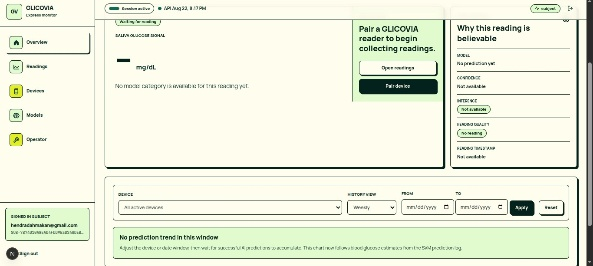
\includegraphics[width=0.8\textwidth]{image7.jpeg}\end{figure}

Gambar 1. Diagram Alir Pelaksanaan Pengembangan Glicovia

\subsection{Persiapan Umum}

Tahap persiapan umum pengembangan prototipe Glicovia bertujuan mengidentifikasi kebutuhan sistem, mengkaji dasar teori, serta merumuskan spesifikasi teknis akhir dari instrumen yang akan dirakit. Pelaksanaan dilakukan di Laboratorium Riset Terpadu Dental Learning Center Fakultas Kedokteran Gigi Universitas Gadjah Mada. Persiapan dimulai dengan diskusi bersama dosen pendamping mengenai mekanisme dan pelaksanaan agenda dari tim PKM-KC. Selanjutnya dilakukan pematangan studi literatur biosensor elektrokimia berbasis saliva menggunakan Screen-Printed Carbon Electrode (SPCE), perancangan sirkuit Analog Front-End khususnya Transimpedance Amplifier (TIA), konversi sinyal digital beresolusi tinggi, serta klasifikasi data dengan algoritma Support Vector Machine (SVM) berbasis Internet of Things (IoT). Pengkajian dilakukan untuk menetapkan dasar teori sebagai landasan dalam merancang prototipe agar sesuai standar dan bisa memenuhi tujuan yang dibutuhkan. Sebelum membuat prototipe, komponen alat dan bahan yang dibutuhkan dibeli secara daring melalui situs belanja online seperti Shopee dan Tokopedia maupun secara luring melalui toko lokal Jogja Karya Techno. Persiapan meliputi desain dan pembuatan Glicovia, rangkaian elektronika, website, dan pelatihan model artificial intelligence. Selain itu, tim rutin mengikuti kegiatan yang diadakan oleh PKM Center Universitas Gadjah Mada seperti, Bukalapak Konsultasi, Sosialisasi, Workshop, serta pelatihan presentasi oleh internal.

\subsection{Perancangan Sistem}

Perancangan Glicovia didasarkan pada kebutuhan dan target luaran pada Bab 1 dan 2 sebagai perangkat portabel skrining prediabetes secara noninvasif.

\subsubsection{Perancangan Perangkat Keras}

Glicovia dirancang sebagai perangkat dengan reader portable untuk deteksi prediabetes. Perangkat keras Glicovia antara lain adalah ESP32 DevKit, SPCE, IC OPA2333, modul ADC ADS1115 (16-bit), serta komponen pasif pendukung. Glicovia didesain dapat membaca sinyal cartridge, mengolah data, dan mengirimkan hasil pada dashboard website ESP32. Cartridge menggunakan Screen-Printed Carbon Electrode (SPCE) melalui adaptor SPCE dan konektor JST untuk mendeteksi glukosa, salivary fructosamine, serta pH saliva. SPCE dan adaptor diperkuat OPA2333 digunakan untuk fabrikasi dan pengujian. Validasi dilakukan bertahap melalui pengujian koneksi, ADC, penguatan sinyal, dan pengujian terintegrasi setelah SPCE serta adaptor tersedia. Komponen prototipe Glicovia secara keseluruhan disajikan pada Gambar 2.

\begin{figure}[h!]\centering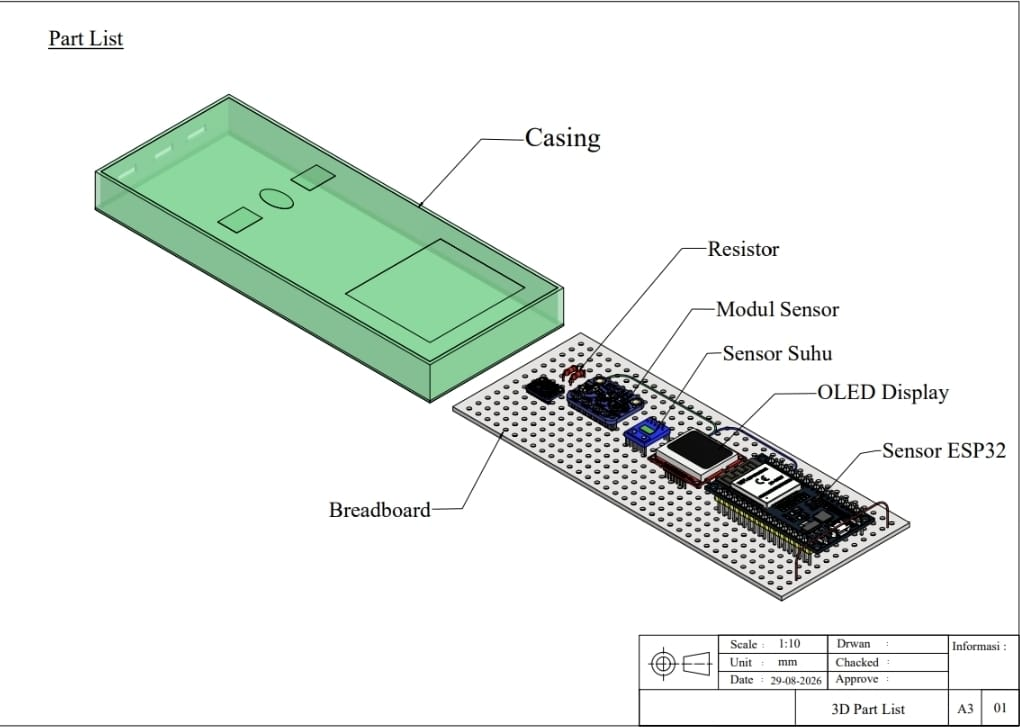
\includegraphics[width=0.8\textwidth]{image2.jpeg}\end{figure}

Gambar 2. Desain Prototipe Glicovia

\subsubsection{Perancangan Perangkat Lunak}

  Pada tahapan membuat perangkat lunak Cardioguard dilakukan pembuatan model AI dan aplikasi mobile. Perangkat lunak Glicovia dirancang modular, meliputi firmware mikrokontroler, pengolahan dan klasifikasi data, API, basis data, serta dashboard web. Data sensor divalidasi berdasarkan nilai kosong, rentang, pencilan, dan gangguan sinyal, kemudian dinormalisasi dan diproses menggunakan SVM kernel radial basis function (RBF). Model menggunakan data glukosa, pH, dan salivary fructosamine dengan standarisasi fitur dan fivefold stratified cross-validation. Kinerja dievaluasi melalui akurasi, macro F1-score, confusion matrix, dan pemeriksaan overfitting, dengan klasifikasi normal, prediabetes, dan diabetes. Data pemeriksaan dikirim melalui BLE atau Wi-Fi, mencakup identitas perangkat, waktu pemeriksaan, biomarka, hasil klasifikasi, dan status validasi menampilkan hasil pemeriksaan, tren biomarka, kategori risiko, riwayat, informasi perangkat, aktivitas operator, serta ekspor laporan PDF.

\subsection{Pembuatan Produk Karsa Cipta/Prototipe}

Realisasi prototipe Glicovia periode ini mencakup validasi desain elektronik, fabrikasi awal cartridge, firmware modular, dan platform web berbasis data sintetis. Simulasi potensiostat menghasilkan settling time 8,2 µs dan bandwidth TIA 1,2 kHz dengan gain flatness ±0,1 dB, sementara dimensi casing terverifikasi mampu mengakomodasi ESP32-S3 DevKit dengan toleransi ±0,2 mm. Cartridge biosensor dirancang menggunakan tiga SPCE terpisah untuk deteksi glukosa (GOx), pH (IrOx), dan fruktosamin (PBA), namun produksi substrat masih tertunda karena pengadaan reagen. Model SVM mencapai waktu inferensi 42 ms. Platform web Next.js 14 telah deployment fungsional dengan skema database Prisma, dashboard zona warna klinis, ekspor PDF, dan validasi batch upload offline. Capaian utama terkonsentrasi pada kematangan desain elektronik, firmware, dan platform digital yang siap integrasi penuh.

Komponen elektronik inti seperti ESP32-WROOM-32U, ADS1115, OPA2333, OLED/LCD I2C, baterai Li-Po, modul TP4056, modul step-up MT3608, tombol, buzzer, konektor JST, breadboard, dan PCB lubang telah tersedia untuk mendukung proses perakitan awal. Sistem kelistrikan dirancang menggunakan baterai Li-Po 3,7 V sebagai sumber daya utama, modul TP4056 untuk pengisian daya, dan MT3608 untuk menaikkan tegangan sesuai kebutuhan komponen. Pada sisi akuisisi sinyal, Glicovia dirancang menggunakan IC OPA2333 sebagai penguat sinyal dan ADS1115 sebagai konverter analog-ke-digital 16-bit sebelum data diproses oleh ESP32. Ta

\subsection{Pengujian}

Prototipe Glicovia telah selesai melalui proses fabrikasi, perakitan, dan pengujian. Pengujian dilakukan untuk memvalidasi desain teknis serta mengkarakterisasi kinerja masing-masing subsistem secara terpisah (component-level testing) sebelum dilakukan pengujian pada tingkat sistem (system-level testing). Setiap subsistem diuji untuk memastikan kesesuaiannya terhadap spesifikasi yang ditetapkan pada Subbab 3.2, sekaligus mengidentifikasi dan meminimalkan potensi kegagalan sebelum dilakukan pengujian secara keseluruhan. Setelah seluruh subsistem memenuhi kriteria yang ditetapkan, prototipe dilanjutkan ke tahap integrasi, kalibrasi, dan pengujian pada tingkat sistem. Seluruh hasil pengujian didokumentasikan dalam lembar hasil uji yang mencakup kondisi pengujian, alat ukur yang digunakan, data hasil pengukuran, serta kesimpulan kelulusan.

Detail protokol dan hasil pengujian disajikan pada Tabel 2.

\begin{longtable}{|p{0.15\textwidth}|p{0.15\textwidth}|p{0.15\textwidth}|p{0.15\textwidth}|}
\hline
Jenis/Komponen yang Diuji & Parameter Uji & Metode Uji & Kriteria Lulus \\
\hline
ESP32-WROOM32U & Fungsi kendali dan komunikasi & Pengujian upload program, pembacaan data serial, serta koneksi Wi-Fi/BLE & ESP32dapat menjalankan program membaca data dan melakukan koneksi nirkabel \\
\hline
Modul ADS111 & Pembacaan sinyal analog & Pemberian tegangan uji bertahap dan pembacaan nilai ADC melalui ESP32 & Tegangan masukan terbaca stabil, keluaran sinyal meningkat serta dikenali oleh ADS1115 tanpa saturasi. \\
\hline
Layar OLED/LCD I2C & Tampilan informasi alat & Pengujian tampilan status alat, nilai sensor, dan hasil klasifikasi & Informasi dapat ditampilkan dengan jelas dan sesuai data yang dikirim ESP32 \\
\hline
Cartridge SPCE & Respons sensor terhadap biomarka saliva & Pengujian menggunakan larutan standar glukosa, pH, dan fruktosamin setelah SPCE tersedia & Sinyal sensor berubah mengikuti variasi konsentrasi atau parameter uji \\
\hline
Sistem klasifikasi & Akurasi & Pengujian & Sistem mampu mengklasifikasikasikan risiko diabetes prediabetes dan non diabetes \\
\hline
\end{longtable}

\section{HASIL YANG DICAPAI}

\subsection{Hasil Luaran PKM-KC}

Luaran PKM-KC Glicovia terdiri atas laporan kemajuan, laporan akhir, prototipe, dan akun media sosial.

\subsubsection{Laporan Kemajuan}

  Laporan kemajuan kegiatan telah disusun dengan capaian sebesar 100\%.

\subsubsection{Laporan Akhir}

  Laporan akhir PKM-KC telah disusun dengan capaian sekitar 65\%.

\subsubsection{Prototipe atau Produk Fungsional yang Telah Tercapai}

Prototipe Glicovia mencapai presentase sekitar 90\%.

\subsubsection{Akun Media Sosial}

Glicovia telah dipromosikan melalui platform media sosial Instagram dan TikTok, dengan menggunakan akun resmi @glicovia.id pada kedua platform tersebut. Terdapat dua postingan yang telah diiklankan (ads) untuk memperoleh jangkauan audiens yang lebih luas. Rincian konten media sosial yang telah dipublikasikan selama pelaksanaan kegiatan disajikan pada Tabel 3. Konten Media Sosial

\begin{longtable}{|p{0.15\textwidth}|p{0.15\textwidth}|p{0.15\textwidth}|p{0.15\textwidth}|}
\hline
No. & Tanggal Unggah & Tautan Konten & Bukti Hasil Unggah \\
\hline
1. & 6 Juni 2026 & Tautan 1 & 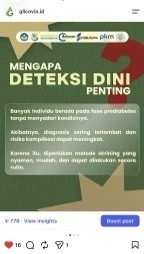
\includegraphics[width=2cm]{image3.jpeg} \\
\hline
2. & 4 Juli 2026 & Tautan 2 & 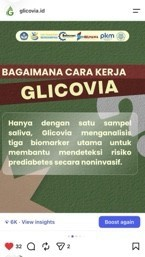
\includegraphics[width=2cm]{image4.jpeg} \\
\hline
3. & 29 Agustus 2026 & Tautan 3 & 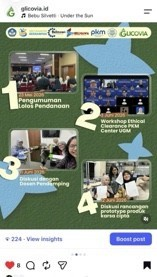
\includegraphics[width=2cm]{image5.jpeg} \\
\hline
\end{longtable}

\subsection{Hasil Luaran Prototipe Produk Karsa Cipta}

Pada periode pelaporan, prototipe Glicovia berada pada tahap realisasi subsistem dan validasi desain komponen. Glicovia telah terealisasikan dengan memanfaatkan mikrokontroler ESP32 DevKit sebagai pusat pengolahan dan pengiriman data. Sinyal elektrokimia yang dideteksi oleh Screen-Printed Carbon Electrode (SPCE) akan diproses melalui rangkaian IC OPA2333 dan ADC ADS1115 16-bit, kemudian dikirimkan oleh ESP32 ke cloud untuk dilakukan analisis. Glicovia dirancang untuk mendeteksi glukosa, salivary fructosamine, dan pH saliva sebagai parameter skrining prediabetes secara noninvasif. Desain teknis telah difinalisasi dan divalidasi melalui simulasi serta pengujian component-level pada Subbab 3.4. Semua subsistem digital, yaitu firmware dan platform web, telah direalisasikan dan diuji secara independen menggunakan mock hardware dan data sintetis.

Model SVM dikembangkan menggunakan metode fivefold stratified cross-validation untuk memastikan kemampuan generalisasi model terhadap data yang digunakan. Kinerja model dievaluasi menggunakan akurasi, macro F1-score, confusion matrix, serta pemeriksaan overfitting dalam mengklasifikasikan hasil pemeriksaan menjadi normal, prediabetes, dan diabetes. Model SVM yang digunakan memiliki waktu inferensi sebesar 42 ms, sehingga memungkinkan proses klasifikasi dilakukan secara cepat setelah data sensor diterima.

Data hasil pemeriksaan yang sudah berada pada cloud akan diakses oleh platform digital Glicovia. Platform Glicovia yang dikembangkan menggunakan Next.js 14 dan basis data Prisma akan menampilkan hasil pemeriksaan berupa nilai biomarker, kategori risiko, waktu pemeriksaan, riwayat pemeriksaan, dan status validasi. Selain itu, platform dilengkapi dengan fitur dashboard zona warna klinis dan ekspor laporan dalam format PDF, sehingga hasil pemeriksaan dapat terdokumentasi dan dipantau secara berkala seperti pada gambar 3.

\begin{figure}[h!]\centering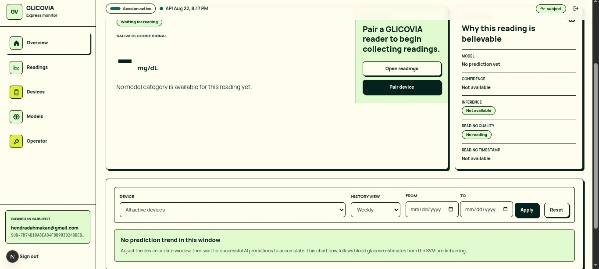
\includegraphics[width=0.45\textwidth]{image6.jpeg}\hfill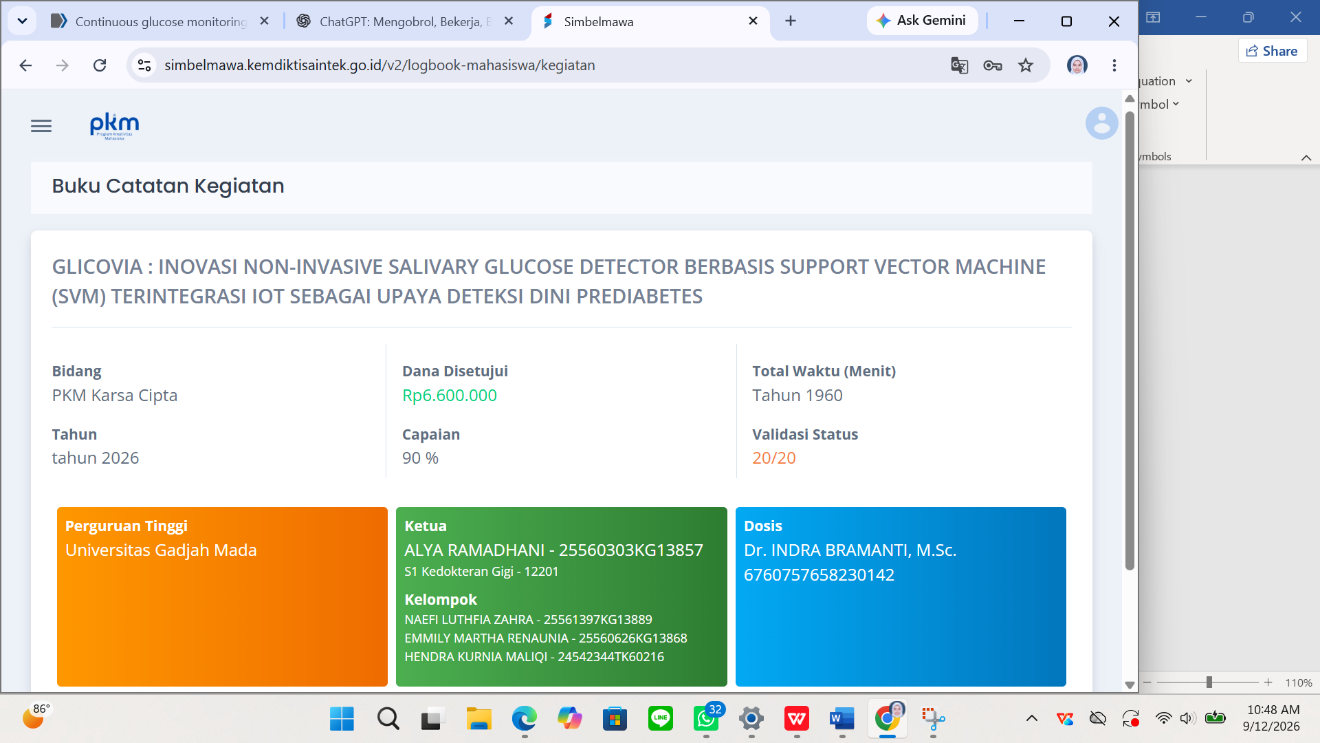
\includegraphics[width=0.45\textwidth]{image29.png}\end{figure}

Gambar 3. Tampilan Platform Digital Glicovia

\section{POTENSI HASIL}

Glicovia memiliki visi jangka panjang sebagai perangkat deteksi dini risiko prediabetes berbasis saliva yang noninvasif dan terintegrasi dengan Internet of Things (IoT). Prototipe saat ini merupakan tahap awal yang masih memerlukan optimalisasi dan validasi bertahap melalui pengujian sensor, evaluasi akurasi dan presisi, validasi terhadap metode standar, serta pengembangan dan validasi model klasifikasi berbasis Support Vector Machine (SVM) untuk memastikan kinerja yang konsisten dan andal. Glicovia akan dikembangkan melalui penyempurnaan sensor, pengolahan data, dan antarmuka digital dengan melibatkan kolaborasi bersama institusi penelitian, fasilitas kesehatan, dan mitra industri. Kebaruan teknologi diarahkan untuk memperoleh perlindungan Hak Kekayaan Intelektual (HKI), meliputi desain perangkat, integrasi sensor dan IoT, serta metode pengolahan data.

Glicovia mendukung SDG 3 (Sustainable Development Goal 3) melalui deteksi dini risiko gangguan metabolik yang lebih nyaman dibandingkan pengambilan darah, sekaligus berpotensi mengurangi penggunaan material habis pakai melalui teknologi noninvasif. Selain itu, Glicovia diharapkan meningkatkan kesadaran masyarakat dengan menyediakan akses skrining prediabetes yang praktis dan mudah digunakan di fasilitas kesehatan, institusi pendidikan dan penelitian, maupun program promotif dan preventif. Implementasinya tetap memerlukan pembuktian kinerja, keamanan, validitas klinis, dan pemenuhan regulasi alat kesehatan. Diseminasi melalui publikasi dan berita juga dilakukan untuk memperluas pemanfaatan hasil, sehingga Glicovia dapat berkembang melalui validasi, perlindungan HKI, hilirisasi, dan diseminasi sebagai teknologi deteksi dini penyakit tidak menular di Indonesia.

\section{RENCANA TAHAPAN BERIKUTNYA}

Rencana tahap selanjutnya yang akan dilaksanakan oleh tim PKM-KC:

1.  Menyelesaikan Laporan Akhir

2.  Membuat poster dan video karsa cipta

3.  Menyelesaikan proses pendaftaran Hak Paten dan desain industri

4.  Melakukan pengujian dan menyempurnakan prototipe hingga selesai 100\%

DAFTAR PUSTAKA

Basilicata, M., Pieri, M., Marrone, G., Nicolai, E., Di Lauro, M., Paolino, V., Tomassetti, F., Vivarini, I., Bollero, P., Bernardini, S. and Noce, A. (2023) ‘Saliva as biomarker for oral and chronic degenerative non-communicable diseases’, Metabolites, 13(8), pp. 889.

Cenzato, N., Cazzaniga, F., Maspero, C., Tartaglia, G. M., \& Del Fabbro, M. (2023) ‘SALIVA-based diagnostic approach for diabetes mellitus: a step towards non-invasive detection–a scoping review’, European Review for Medical and Pharmacological Sciences, 27(24), pp. 12080–12087.

Chawang, K., Bing, S., Kwon, K. Y., \& Chiao, J.-C. (2024). ‘Miniaturized iridium oxide microwire pH sensor for biofluid sensing’, Chemosensors, 12(8), pp. 168.

Ferdina, A. R., Juhairiyah, Yuana, W. T., Setyawati, B., \& Pangestika, D. E. (2025). ‘Sociodemographic and Lifestyle Factors Associated with Undiagnosed Diabetes in Indonesia: Findings from the Basic Health Research Work of Riskesdas 2018’, Journal of the ASEAN Federation of Endocrine Societies, 40(1), pp. 53–60.

Hall, J.E. (2021) Guyton and Hall Textbook of Medical Physiology. 14th Edition Philadelphia: Elsevier.

Holt E, Nguyen H, Bispham J, Liu J, Chapman K, Grady M. (2023) ‘Perceptions of Continuous Glucose Monitoring Systems in the T1D Exchange Diabetes Registry: Satisfaction, Concerns, and Areas for Future Improvement.’ Clin Diabetes. 42(1) pp. 104-115.

International Diabetes Federation (2025) IDF Diabetes Atlas. 11th Edition. Brussels: International Diabetes Federation. Tersedia di: https://diabetesatlas.org/ (Diakses: 25 Juni 2026).

International Organization for Standardization (2016), ISO 13485:2016: Medical devices—Quality management systems—Requirements for regulatory purposes. Tersedia di: https://www.iso.org/standard/59752.html? utm_source=chatgpt.com

International Organization for Standardization (2025), ISO 10993-1:2025: Biological evaluation of medical devices—Part 1: Requirements and general principles for the evaluation of biological safety within a risk management process. Tersedia di: https://www.iso.org/standard/10993-1?browse=tc\&utm_source=chatgpt.com

Kumar, V., Abbas, A., K. and Aster, J.C. (2020) Robbins \& Cotran Pathologic Basis of Disease. 10th Edition. Philadelphia: Elsevier.

  Thapa, M., \& Heo, Y. S. (2025). Label-free Electrochemical Biosensor for Glycated Hemoglobin (HbA1c) and Glycated Albumin (GA) Measurement Using 4-mercapto-phenyl Boronic Acid Embedded Affinity. BioChip Journal, 19(2), 248–261.

Vabalas, A., Gowen, E., Poliakoff, E., \& Casson, A. J. (2019) ‘Machine learning algorithm validation with a limited sample size’, PLOS ONE, 14(11), e0224365.

LAMPIRAN

Lampiran 1. Penggunaan Dana

  Lampiran 1.1Rekap Penerimaan Dana

\begin{longtable}{|p{0.15\textwidth}|p{0.15\textwidth}|p{0.15\textwidth}|p{0.15\textwidth}|}
\hline
No. & Sumber Pemasukan & Jenis Dana & Jumlah (Rp) \\
\hline
1. & Belmawa & In-cash & 5.940.000 \\
\hline
2. & PT (UGM) & In-cash + Inkind & 1.500.000 \\
\hline
\end{longtable}

  Lampiran 1.2Rincian penggunaan dana (total in-cash Belmawa)

\begin{longtable}{|p{0.15\textwidth}|p{0.15\textwidth}|p{0.15\textwidth}|p{0.15\textwidth}|p{0.15\textwidth}|}
\hline
No. & Jenis Pengeluaran & Volume & Harga Satuan (Rp) & Total (Rp) \\
\hline
1. & Belanja Bahan (maks. 60\%) &  &  &  \\
\hline
 & Enzim Glukosa Oksidase 50 gram & 1 & 172.200 & 172.200 \\
\hline
 & Adapter Connector Screen Printed Electrode & 3 & 215.000 & 645.000 \\
\hline
 & Kabel Jumper Male Female 40pcs 20cm 2.54mm Breadboard Arduino & 1 & 10.500 & 10.500 \\
\hline
 & Antenna Wifi 2.4Ghz 2.4Ghz Antena Pigtail S MA ESP 32 ESP32 Nodemcu & 2 & 18.900 & 37.800 \\
\hline
 & Box Storage Plastik Tempat Komponen Aksesoris & 1 & 30.000 & 30.000 \\
\hline
 &  &  &  &  \\
\hline
 & Adapter Plate SOP8 SO8 SOIC8SSOP8to DIP DIP8 PCB Converter & 10 & 1.000 & 10.000 \\
\hline
 & Modul LCD Display 1602 White On Blue With I2C SPI Backpack Module & 2 & 30.000 & 60.000 \\
\hline
 & Pin 1x40Pin Female Header Single Row 2.54 mm & 5 & 1.900 & 9.500 \\
\hline
 & Kabel Jumper Female Female 40pcs 20cm 2.54mm Breadboard Arduino & 1 & 10.000 & 10.000 \\
\hline
 & Pinset Lurus Bengkok Relife TS-11TS-15 & 1 & 21.500 & 21.500 \\
\hline
 & Pinset Lurus/Bengkok Relife TS-15 & 1 & 21.500 & 21.500 \\
\hline
 & Konektor Kabel JST Quick Connector 2P 3P 5P 6P Aristo Style & 5 & 2.300 & 11.500 \\
\hline
 & Tactile Switch Waterproof 12x12x10mm 4Pin & 10 & 2.000 & 20.000 \\
\hline
 & Kabel Jumper Male - Male 40pcs 20cm 2.54mm Breadboard Arduino & 1 & 11.000 & 11.000 \\
\hline
 & Buzzer Aktif 5V & 5 & 3.000 & 15.000 \\
\hline
 & Paket Kapasitor Keramik & 1 & 52.040 & 52.040 \\
\hline
 & Paket Resistor Pack 1/4W 0.25Watt 1\% 1\% Metal Film 30Nilai & 1 & 30.000 & 30.000 \\
\hline
 & Kotak Perkakas Plastik & 1 & 159.701 & 159.701 \\
\hline
 & Solderless Breadboard MB- 102 & 3 & 12.000 & 36.000 \\
\hline
 & ESP32DevkitC V4ESP Wroom 32D 32U Development Board & 3 & 79.500 & 238.500 \\
\hline
 & Baterai Pouch Universal LiPo 3.7V 1200mAh Tanpa Soket & 1 & 60.160 & 60.160 \\
\hline
 & PALO Baterai Universal & 1 & 105.040 & 105.040 \\
\hline
 &  &  &  &  \\
\hline
 & MT3608DC-DC 2A Step Up Boost Converter Module Mini Power Booster & 5 & 7.300 & 36.500 \\
\hline
 & Fan 9cm 90mm 92mm 12v DC Kipas Komputer PC CPU Case Casing Heatsink & 1 & 17.900 & 17.900 \\
\hline
 & Kabel 26AWG UL100726 AWG Electronic PVC Insulated Wire AWG 26UL 1007 & 2 & 1.500 & 3.000 \\
\hline
 & Heatshrink Tube Set & 1 & 45.900 & 45.900 \\
\hline
 & PCB Lubang Prototype 2.54mm FR4Double Layer Hijau & 5 & 7.700 & 38.500 \\
\hline
 & Kabel 26AWG UL100726 AWG Electronic PVC Insulated Wire AWG 26UL 1007 & 2 & 1.500 & 3.000 \\
\hline
 & Oled 1.3inch White Blue 128x64LCD I2C Display Putih Biru & 2 & 44.500 & 89.000 \\
\hline
 & 1x40Pin Male Header Single Row 2.54mm & 5 & 1.500 & 7.500 \\
\hline
 & Tenol Timah Solder Paragon & 1 & 36.000 & 36.000 \\
\hline
 & ADS111516bit I2C 4 Channel ADC - PGA & 3 & 26.000 & 78.000 \\
\hline
 & Flux Paste Pasta Solder IC CPU Bebas Timbal – Relife HW1110CC & 1 & 38.000 & 38.000 \\
\hline
 & Kabel 26AWG UL100726 AWG Electronic PVC Insulated Wire AWG 26UL 1007 & 2 & 1.500 & 3.000 \\
\hline
 & Modul TP4056Protect USB Type C Charger Baterai Lithium 18650Charging & 5 & 3.300 & 16.500 \\
\hline
 & Konektor JST PH2.0PH & 20 & 500 & 10.000 \\
\hline
 &  &  &  &  \\
\hline
 & Zoyi Kabel Jarum Multitester Set 10A CAT II 1000V 600V & 1 & 43.764 & 43.764 \\
\hline
 & Goot Wick 2.0MM Original & 1 & 25.552 & 25.552 \\
\hline
 & Kabel 26AWG UL100726 AWG Electronic PVC Insulated Wire AWG 26UL 1007 & 2 & 1.500 & 3.000 \\
\hline
 & Ultra-Low Capacitance Double Rail-to-Rail ESD Protection Diode & 5 & 7.299 & 36.495 \\
\hline
 & Modul TCRT5000Infrared IR Line Tracking Tracing Sensor & 5 & 6.000 & 30.000 \\
\hline
 & Two-Channel 1.8V microPower CMOS Operational Amplifier Zero-Drift Series & 3 & 28.946 & 86.838 \\
\hline
 & Screen Printed Electrode SPE & 16 & 208.566 & 625.700 \\
\hline
 & PH Tester Digital Pocket & 1 & 48.035 & 48.035 \\
\hline
 & Serbuk Kalibrasi PH Buffer & 1 & 6.000 & 6.000 \\
\hline
 & Eppendorf Tube 2mL & 150 & 1.500 & 225.000 \\
\hline
 & Glukometer & 1 & 228.250 & 228.250 \\
\hline
 & Sarung tangan medis & 1 & 37.996 & 31.996 \\
\hline
 & True RMS Avometer & 1 & 212.373 & 212.373 \\
\hline
SUB TOTAL &  &  &  & Rp3.792.744 \\
\hline
2. & Belanja Sewa (maks. 15\%) &  &  &  \\
\hline
 & Sewa akses jurnal (maksimal 6bulan) & 1 & 100.000 & 100.000 \\
\hline
 & Ethical Clearance & 1 & 165.000 & 165.000 \\
\hline
 & Desain 3D Printing & 1 & 280.000 & 280.000 \\
\hline
 & Sewa lab (termasuk penggunaan alat lab) & 1 & 300.000 & 300.000 \\
\hline
SUB TOTAL &  &  &  & 845.000 \\
\hline
3. & Perjalanan lokal (maks. 30\%) &  &  &  \\
\hline
 & Kegiatan pendampingan & 1 & 602.500 & 602.500 \\
\hline
 & Dana transportasi & 4 & 100.000 & 400.000 \\
\hline
SUB TOTAL &  &  &  & 1.002.500 \\
\hline
4. & Lain-lain (maks. 15\%) &  &  &  \\
\hline
 & Adsense akun media sosial (maks. 500.000) & 3 & 50.897 & 152.691 \\
\hline
 & Percetakan produk & 1 & 194.000 & 194.000 \\
\hline
 & Publikasi Berita & 1 & 100.000 & 100.000 \\
\hline
 & Dana akses data dan & 4 & 100.000 & 400.000 \\
\hline
 &  &  &  &  \\
\hline
 & SUB TOTAL &  &  & 846.691 \\
\hline
GRAND TOTAL &  &  &  & 6.486.935 \\
\hline
GRAND TOTAL: Enam Juta Empat Ratus Delapan Puluh Enam Ribu Sembilan Ratus Tiga Puluh Lima Rupiah &  &  &  &  \\
\hline
\end{longtable}

  Lampiran 1.3Bukti Penggunaan Dana

\begin{longtable}{|p{0.15\textwidth}|p{0.15\textwidth}|p{0.15\textwidth}|}
\hline
No. & Bukti Penggunaan Dana & Keterangan \\
\hline
1. & 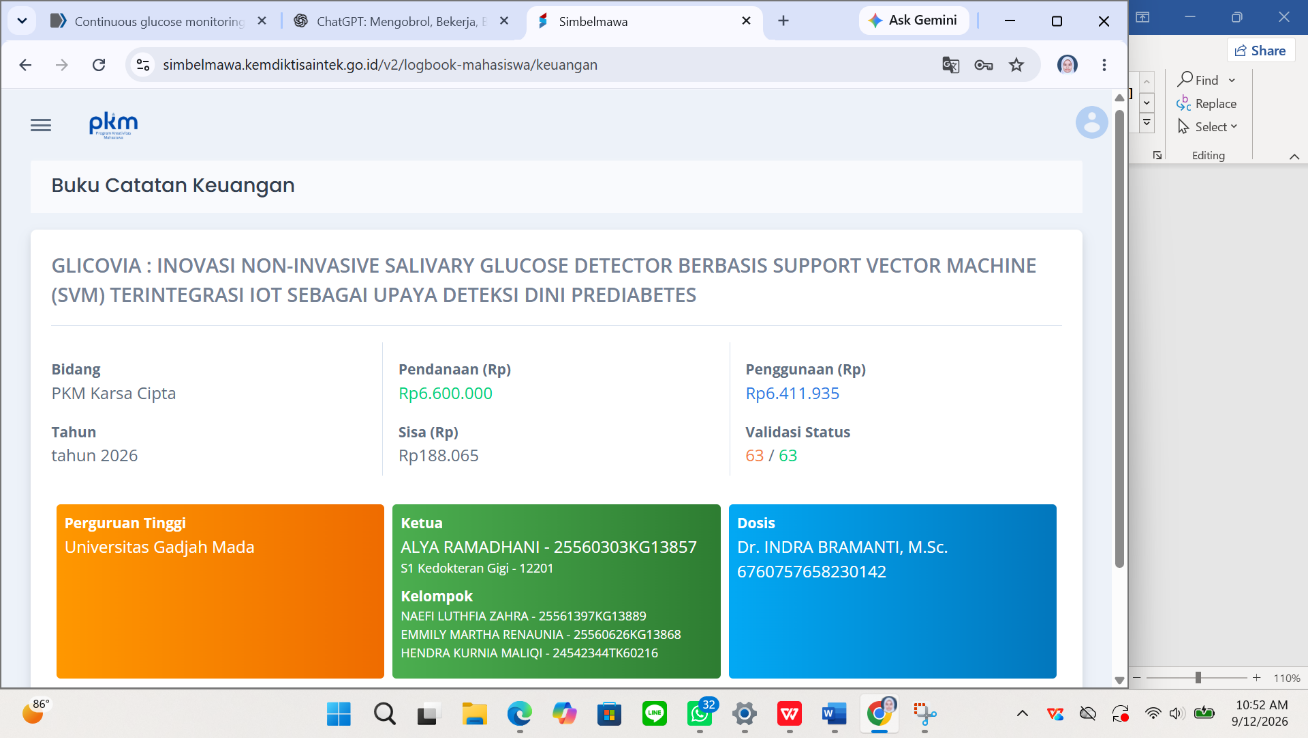
\includegraphics[width=2cm]{image30.png} & Tanggal: 10 September 2026 Penggunaan: Pembelian bahan SPCE sebagai cartridge biosensor Pembeli: Naranabil Daffa Iskandar \\
\hline
2. & 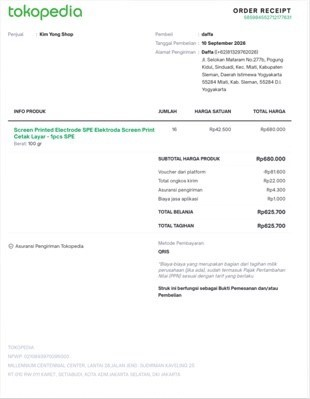
\includegraphics[width=2cm]{image8.jpeg} & Tanggal: 5 September 2026 Penggunaan: Enzim GOx untuk uji kalibrasi alat Pembeli: Alya Ramadhani \\
\hline
3. & 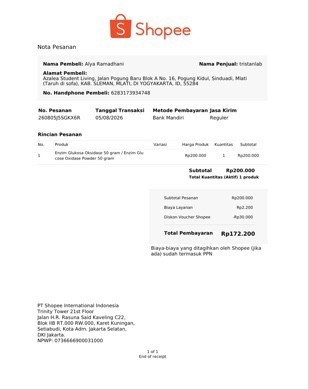
\includegraphics[width=2cm]{image9.jpeg}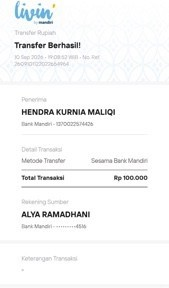
\includegraphics[width=2cm]{image10.jpeg} & Tanggal: 10 Agustus 2026 Penggunaan: Pembelian kuota internet anggota tim Pembeli: Alya Ramadhani \\
\hline
 &  &  \\
\hline
 & 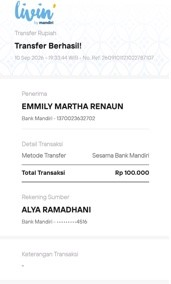
\includegraphics[width=2cm]{image11.jpeg} &  \\
\hline
4. & 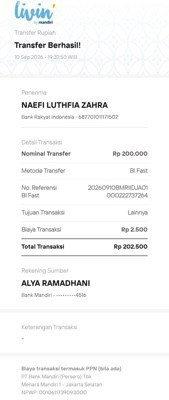
\includegraphics[width=2cm]{image12.jpeg} & Tanggal: 9 Agustus 2026 Penggunaan: Pembelian PH Tester Digital Pocket-Sized pH Meter PH- 009(I)A untuk uji kalibrasi Pembeli: Hendra Kurnia Maliki \\
\hline
5. & 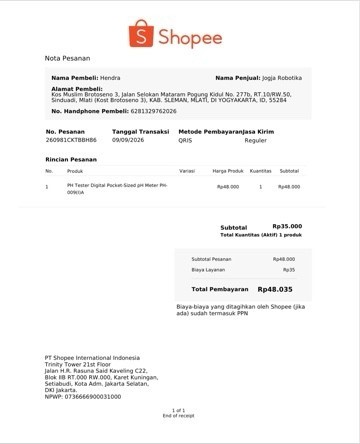
\includegraphics[width=2cm]{image13.jpeg} & Tanggal: 29 Agustus 2026 Penggunaan: Pengeluaran untuk pemasangan iklan berbayar (Instagram Ads) guna mendukung publikasi dan sosialisasi program PKM kepada masyarakat. Pembeli: Alya Ramadhani \\
\hline
6. & 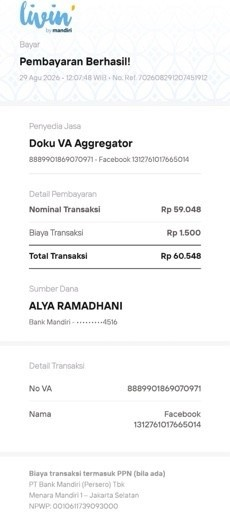
\includegraphics[width=2cm]{image14.jpeg} & Tanggal: 11 Agustus 2026 Penggunaan: Pembuatan otak utama algoritma AI Pembeli: Narabil Daffa Iskandar \\
\hline
 &  &  \\
\hline
7. & 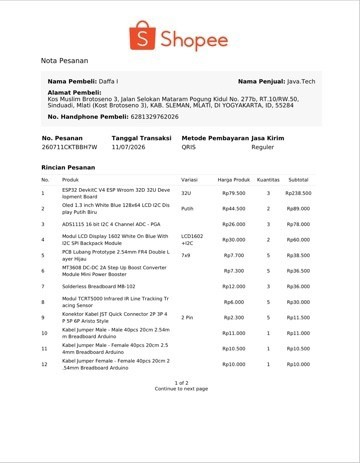
\includegraphics[width=2cm]{image15.jpeg} & Tanggal: 9 September 2026 Penggunaan: Glukometer sebagai perbandingan validasi hasil pengecekan glukosa saliva Pembeli: Naefi Luthfia Zahra \\
\hline
 &  &  \\
\hline
\end{longtable}

Lampiran 2. Bukti-bukti Pendukung Kegiatan

  Lampiran 2.1 Bukti aktivitas

\begin{figure}[h!]\centering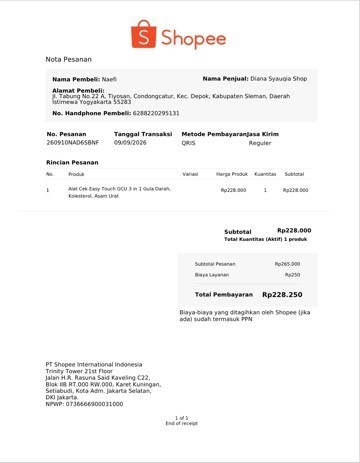
\includegraphics[width=0.8\textwidth]{image16.jpeg}\end{figure}

  Gambar 1. Pembuatan Desain Prototipe

\begin{figure}[h!]\centering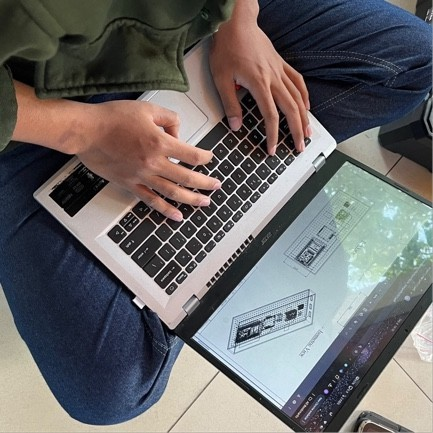
\includegraphics[width=0.8\textwidth]{image17.jpeg}\end{figure}

  Gambar 2. Proses Perakitan Elektronis

\begin{figure}[h!]\centering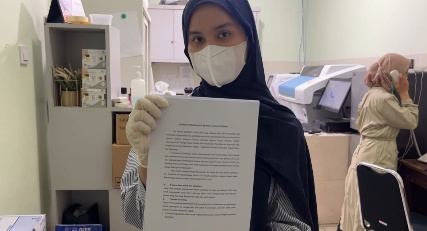
\includegraphics[width=0.8\textwidth]{image21.jpeg}\end{figure}

  Gambar 3. Proses Kalibrasi Alat

\begin{figure}[h!]\centering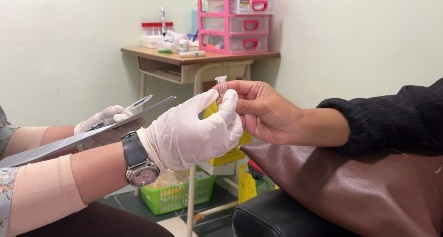
\includegraphics[width=0.45\textwidth]{image22.jpeg}\hfill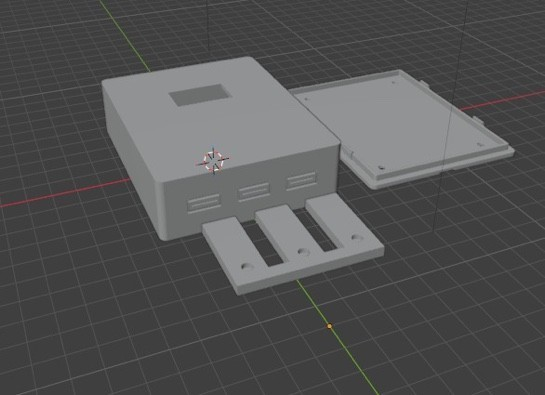
\includegraphics[width=0.45\textwidth]{image24.jpeg}\end{figure}

\begin{figure}[h!]\centering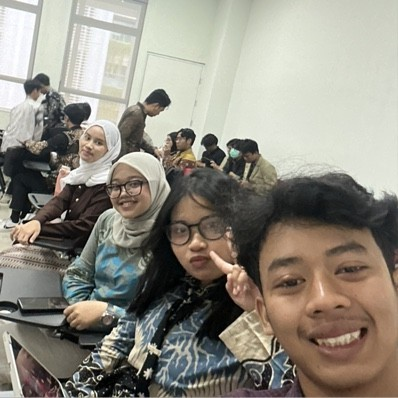
\includegraphics[width=0.8\textwidth]{image25.jpeg}\end{figure}

Gambar 4. Pengujian Hasil

\begin{figure}[h!]\centering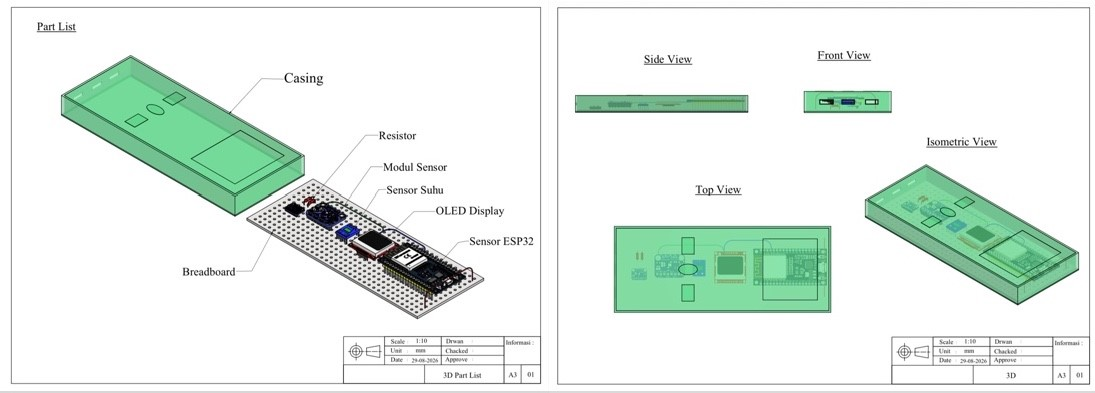
\includegraphics[width=0.8\textwidth]{image23.jpeg}\end{figure}

  Gambar 5. Hasil Desain Prototipe

\begin{figure}[h!]\centering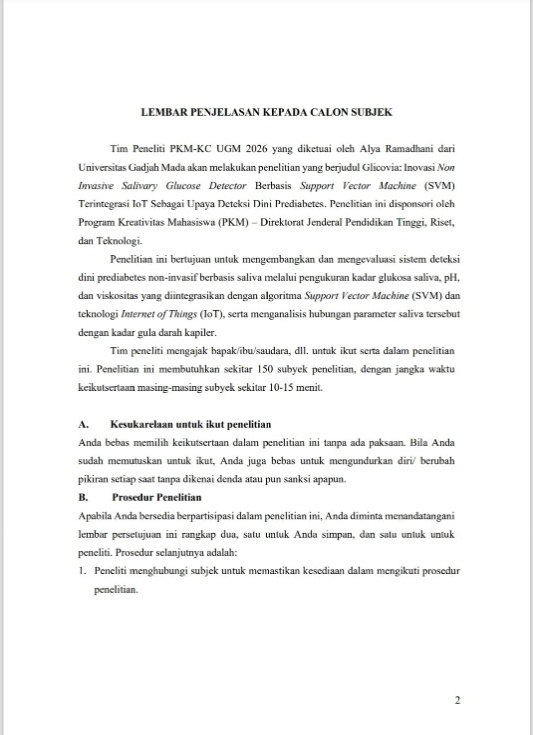
\includegraphics[width=0.8\textwidth]{image32.jpeg}\end{figure}

  Gambar 6. Pembuatan Desain 3D Printing

\begin{figure}[h!]\centering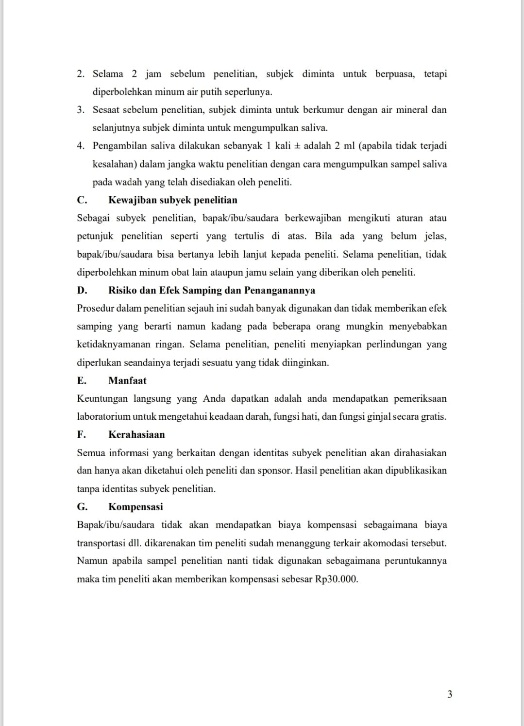
\includegraphics[width=0.8\textwidth]{image33.jpeg}\end{figure}

  Gambar 7. Diskusi Internal Tim

\begin{figure}[h!]\centering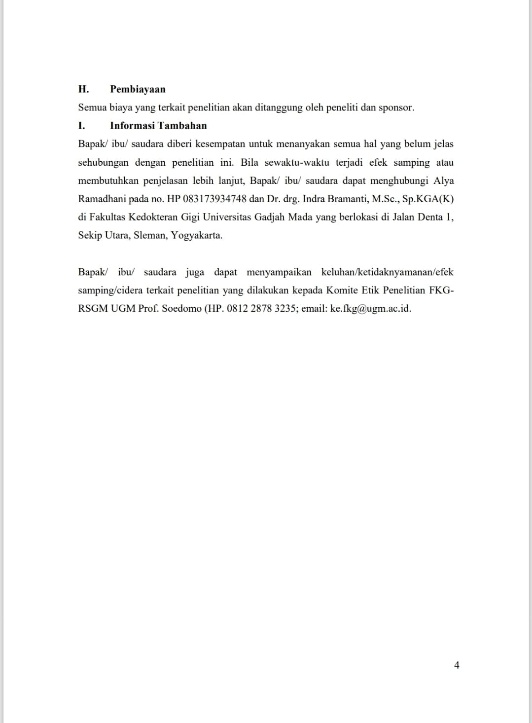
\includegraphics[width=0.45\textwidth]{image34.jpeg}\hfill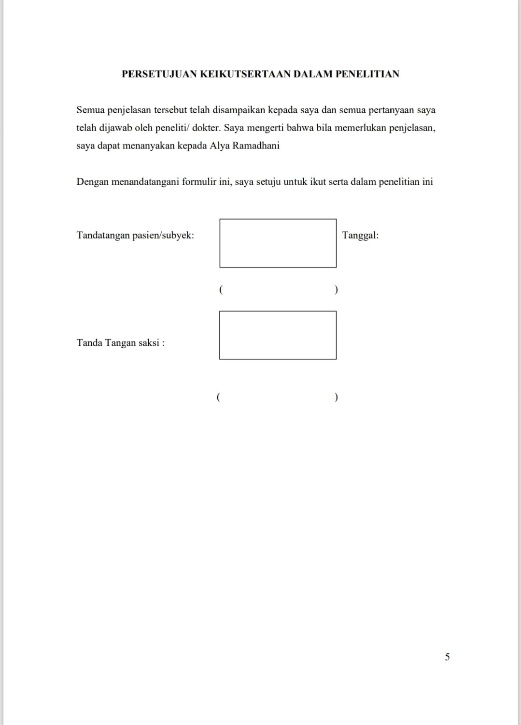
\includegraphics[width=0.45\textwidth]{image35.jpeg}\end{figure}

Gambar 8. Diskusi dengan Dosen Pembimbing

\begin{figure}[h!]\centering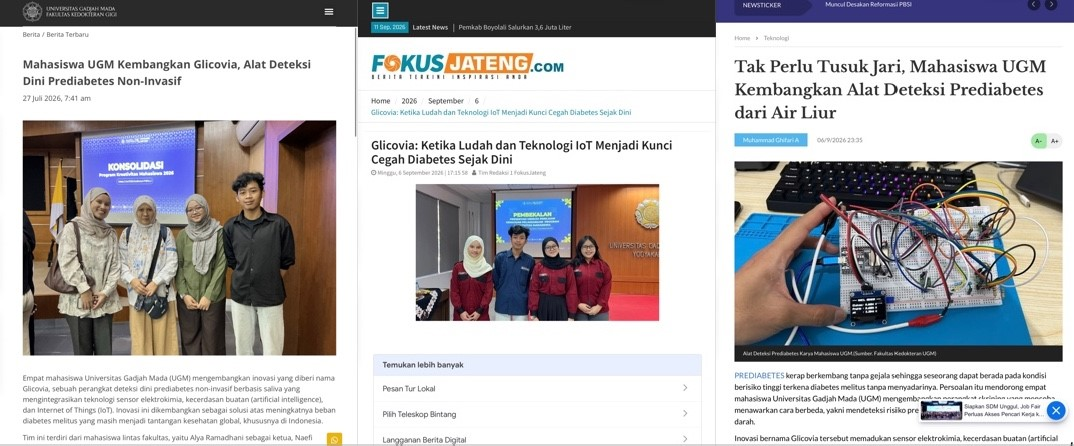
\includegraphics[width=0.8\textwidth]{image36.jpeg}\end{figure}

Gambar 9. Diskusi dengan laboran Gadjah Mada Medical Center

  Lampiran 2.2 Screenshoot gambar pengisian log book

\begin{figure}[h!]\centering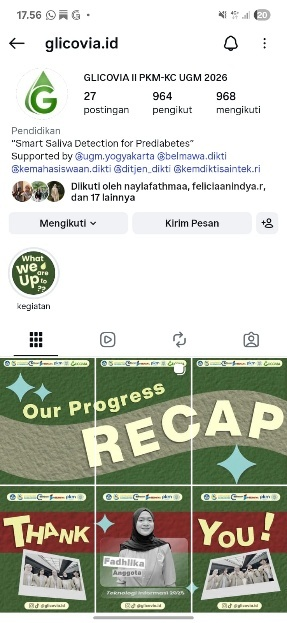
\includegraphics[width=0.8\textwidth]{image37.jpeg}\end{figure}

  Gambar 10. Log Book Kegiatan

\begin{figure}[h!]\centering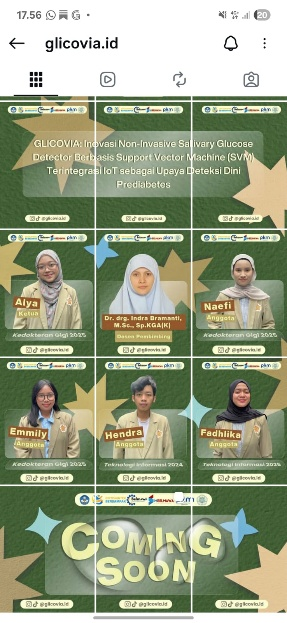
\includegraphics[width=0.8\textwidth]{image38.jpeg}\end{figure}

  Gambar 11. Log Book Keuangan Lampiran

Lampiran 2.3 Ethical Clearance

\begin{figure}[h!]\centering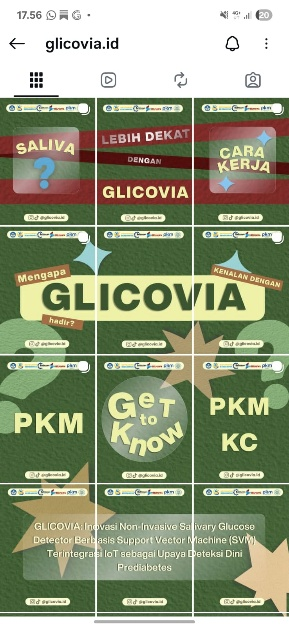
\includegraphics[width=0.8\textwidth]{image39.jpeg}\end{figure}

Lampiran 2.4 Formulir Informed Consent

\begin{figure}[h!]\centering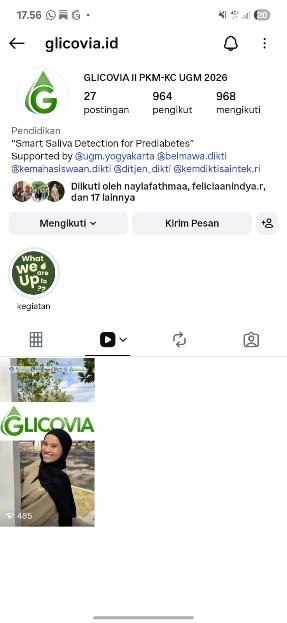
\includegraphics[width=0.45\textwidth]{image40.jpeg}\hfill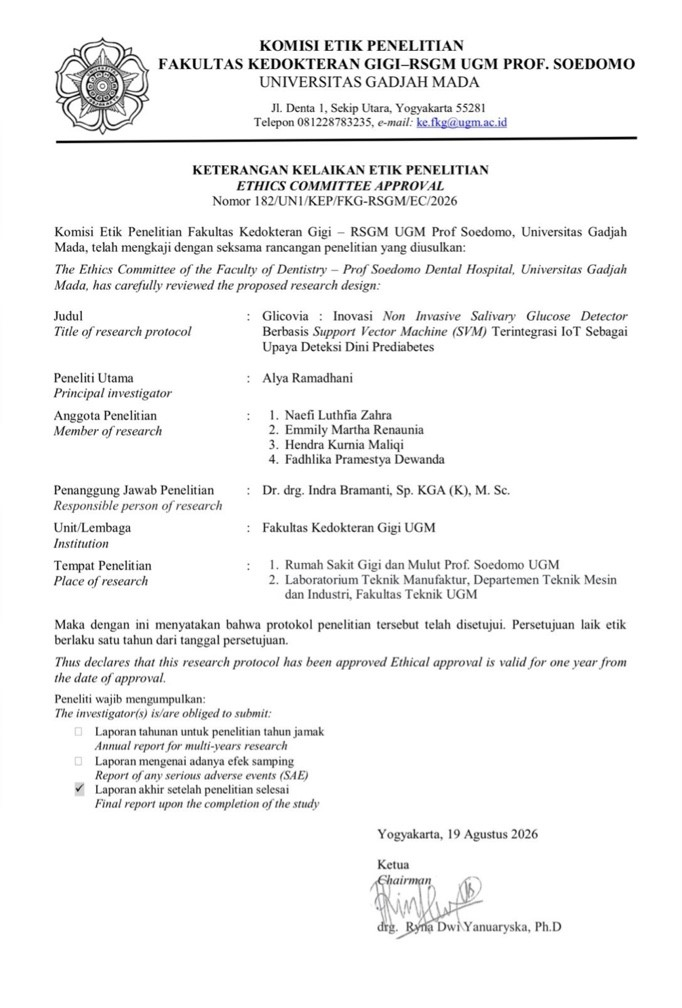
\includegraphics[width=0.45\textwidth]{image31.jpeg}\end{figure}

\begin{figure}[h!]\centering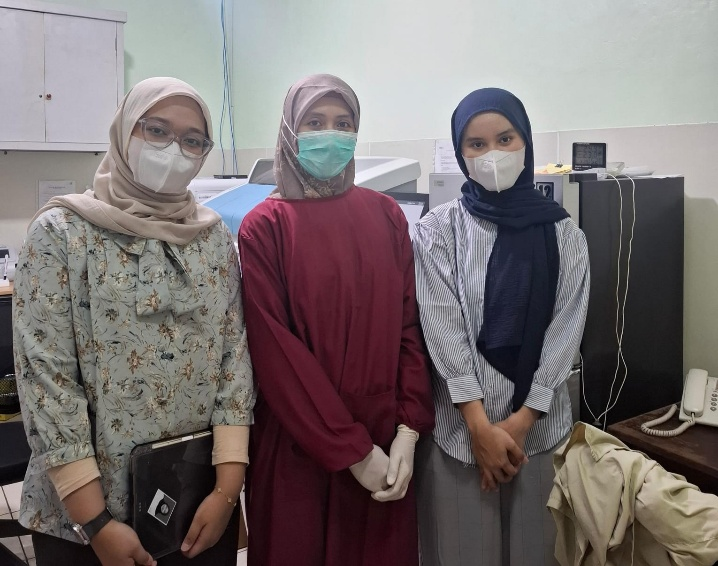
\includegraphics[width=0.45\textwidth]{image28.jpeg}\hfill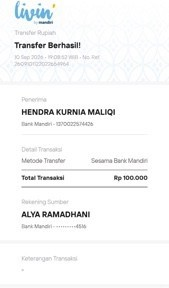
\includegraphics[width=0.45\textwidth]{image100.jpeg}\end{figure}

Lampiran 2.5 Publikasi Artikel

\begin{figure}[h!]\centering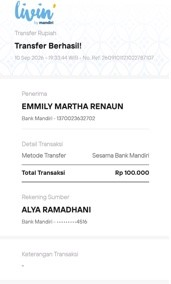
\includegraphics[width=0.8\textwidth]{image110.jpeg}\end{figure}

Lampiran 2.6 Akun Media Sosial

\begin{figure}[h!]\centering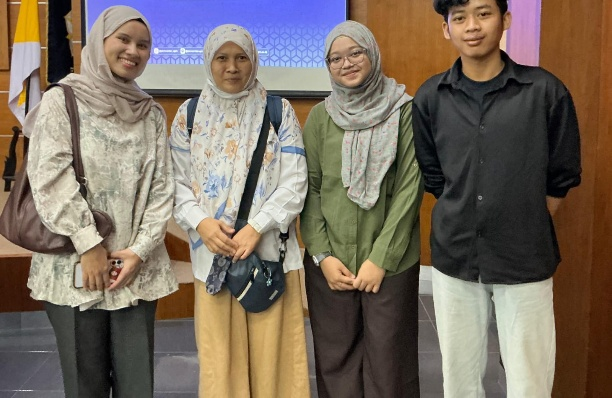
\includegraphics[width=0.22\textwidth]{image27.jpeg}\hfill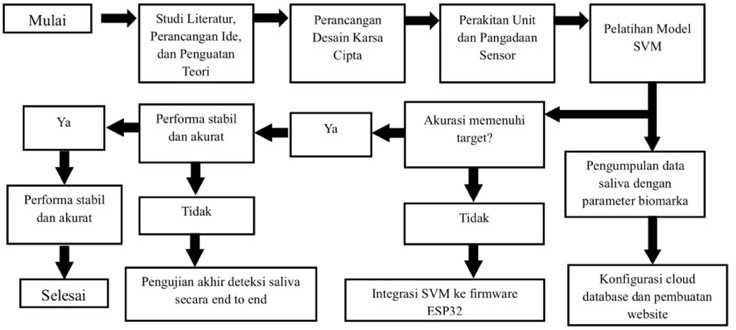
\includegraphics[width=0.22\textwidth]{image1.jpeg}\hfill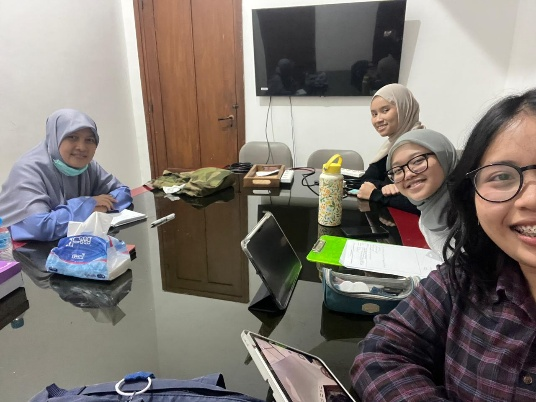
\includegraphics[width=0.22\textwidth]{image26.jpeg}\hfill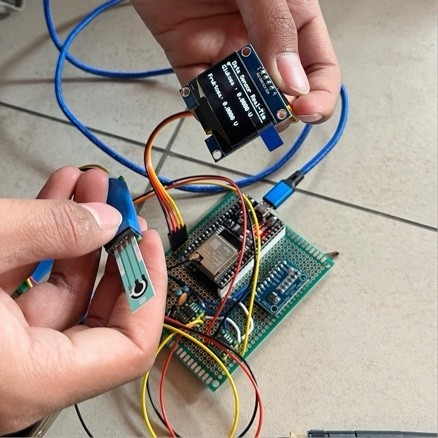
\includegraphics[width=0.22\textwidth]{image19.jpeg}\end{figure}

  24

\end{document}
